\section{CHAPTER 8: TRAPS AND CONTROL VALVES}
\subsection{Acquaintance}
Steam traps and control valves are essential components in industrial steam systems. Steam traps are automatic valves designed to remove condensate (condensed steam and non-condensable gases) without letting steam escape. Control valves, on the other hand, are used to regulate the flow and pressure of steam, ensuring optimal performance and safety in various industrial processes. Together, these components play a crucial role in maintaining efficiency and preventing energy wastage in steam systems.

\subsection{Types of Steam Traps}
\subsubsection{Single Orifice Float Trap}

\textbf{Description:} The Forbes Marshall Single Orifice Float Trap is a condensate drain trap with a single orifice, optimal for process applications.
\begin{figure}[h]
    \centering
    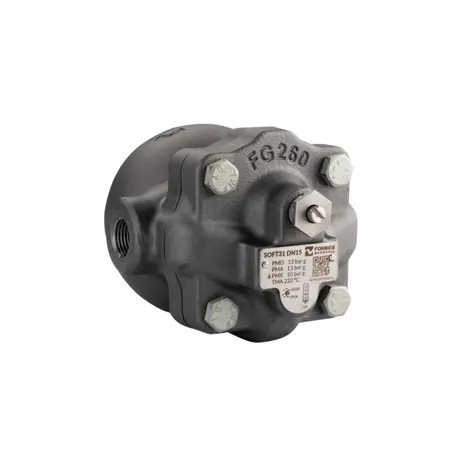
\includegraphics[width=0.8\textwidth,height=0.33\textheight,keepaspectratio]{figs/lastmin/Single Orifice Ball Float Trap.png}
    \caption{Single Orifice Float Trap}
    \label{fig:single_orifice_float_trap}
\end{figure}

\textbf{Features:}
\begin{enumerate}
    \item Efficient drainage of condensate.
    \item There is no steam loss during regular operations, reducing the carbon footprint.
    \item Erosion deflectors with simplified flow paths enhance resistance to erosion and impact.
    \item Self-aligning primary valve and water hammer-resistant float assembly.
\end{enumerate}
\subsubsection{Compact Module Two Orifice Float Trap}

\textbf{Description:} This trap is engineered to manage substantial discharge capacity during system initiation and peak condensate loads.

\begin{figure}[h]
    \centering
    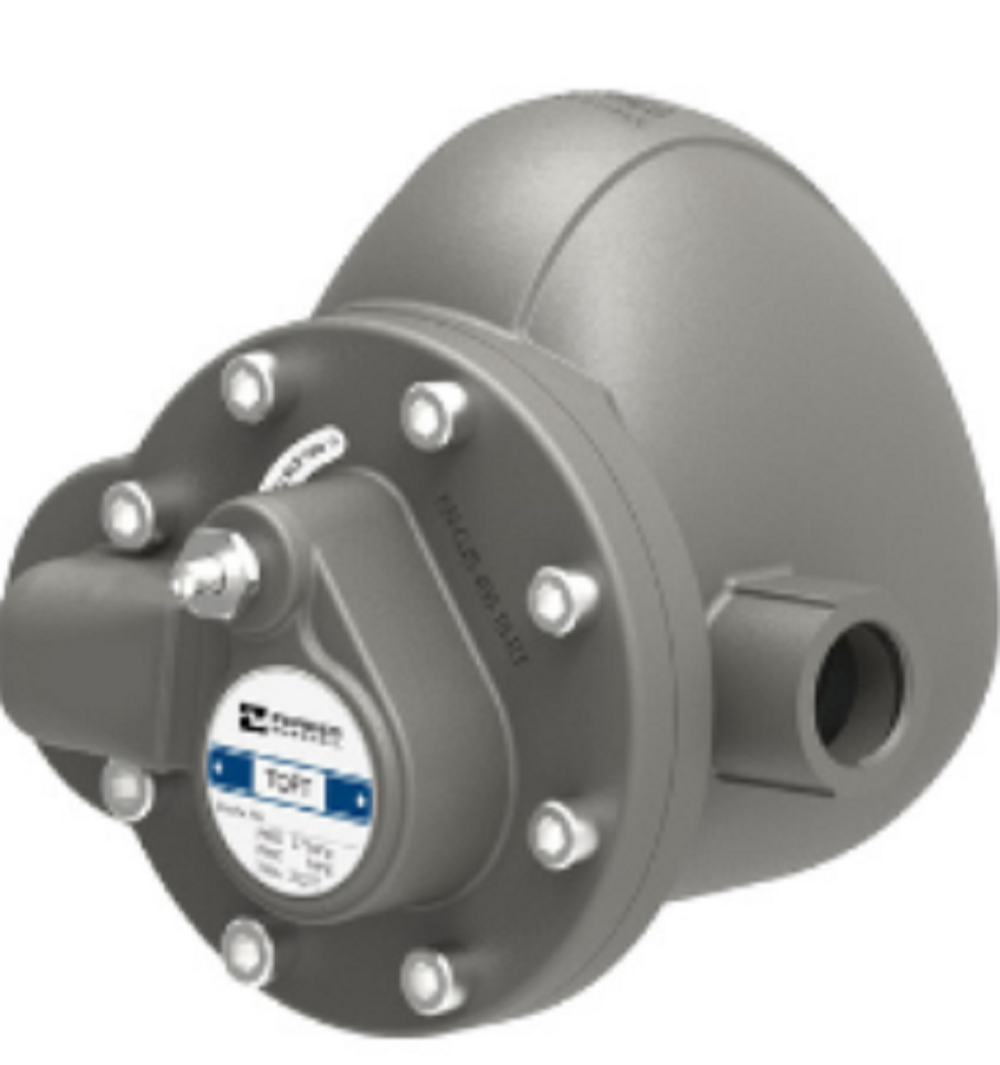
\includegraphics[width=0.8\textwidth,height=0.33\textheight,keepaspectratio]{figs/lastmin/two_orific_float_trap.png}
    \caption{Compact Module Two Orifice Float Trap}
    \label{fig:compact_module_two_orifice_float_trap}
\end{figure}

\textbf{Features:}
\begin{enumerate}
    \item Dual orifice system is controlled by a lever and float mechanism.
    \item Integrated air vent and steam lock release mechanism.
    \item Compact design with a strainer, non-return valve, inlet, outlet, and float.
    \item Piston valves to prevent loss in the inline due to the gland.
\end{enumerate}
\subsubsection{Thermodynamic Trap}

\textbf{Description:} Forbes Marshall Thermodynamic Steam Traps are known for their superior resistance to corrosion and effective condensate removal.

\begin{figure}[h]
    \centering
    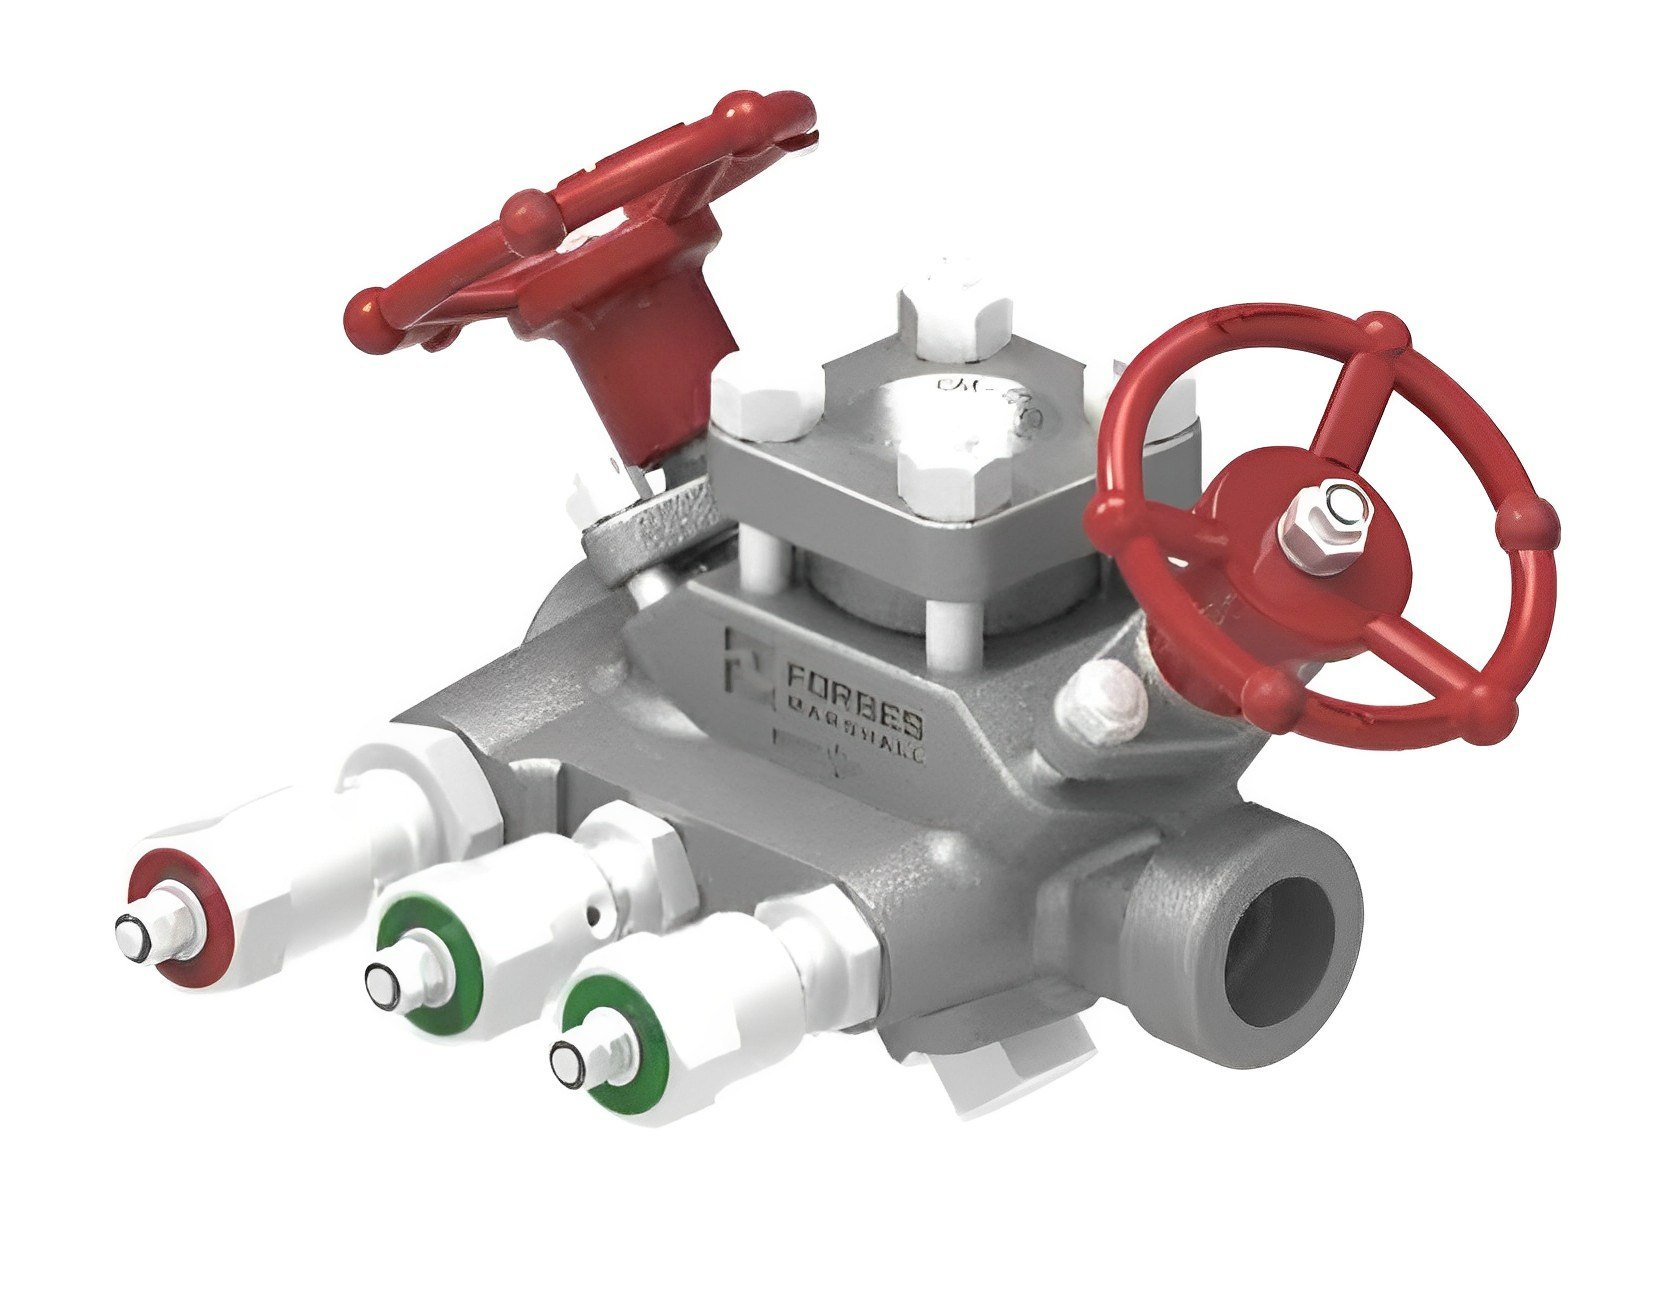
\includegraphics[width=0.8\textwidth,height=0.33\textheight,keepaspectratio]{figs/lastmin/thermodynamic_trap.png}
    \caption{Thermodynamic Trap}
    \label{fig:thermodynamic_trap}
\end{figure}

\textbf{Features:}
\begin{enumerate}
    \item Various sizes and end connections are available for installation flexibility.
    \item Anti-air binding discs are available upon request.
    \item Suitable for all pressure ranges.
    \item Induction-hardened seating area for an extended lifespan.
\end{enumerate}
\subsubsection{Compact Module Thermodynamic Trap}

\textbf{Description:} This module integrates a thermodynamic steam trap with a pipeline connector through a universal connector.

\textbf{Features:}
\begin{enumerate}
    \item In-line components for easy specification and installation.
    \item Forged carbon steel construction for longevity.
    \item Quick installation process, taking less than 45 minutes.
    \item Can be installed in any angular direction without an angled trap position.
\end{enumerate}
\subsubsection{Bimetallic Trap}

\textbf{Description:} The Bimetallic Steam Trap, designed by Forbes Marshall, efficiently discharges steam lines operating at high pressure and temperature levels.
\begin{figure}[h]
    \centering
    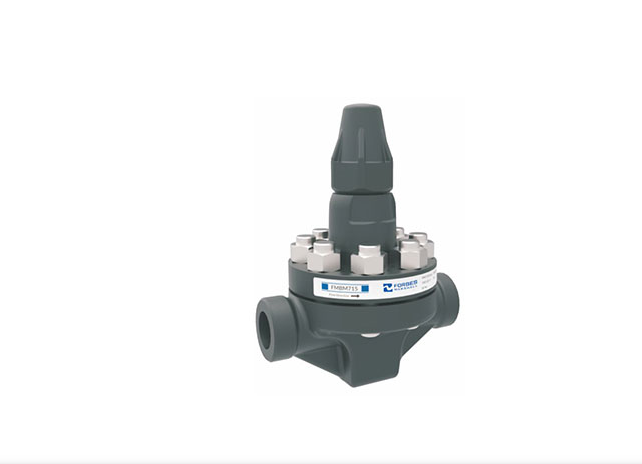
\includegraphics[width=0.8\textwidth,height=0.33\textheight,keepaspectratio]{figs/lastmin/bimetallic_thermostatic_steam_trap.png}
    \caption{Bimetallic Trap}
    \label{fig:bimetallic_trap}
\end{figure}


\textbf{Features:}
\begin{enumerate}
    \item Stainless steel insert for resilience against erosion and corrosion.
    \item Condensate section with a check valve for precise control.
    \item Integrated strainer screen for debris filtration.
    \item External adjustment screw for regulating discharge temperature.
\end{enumerate}
\subsubsection{Bucket Traps}

\textbf{Description:} Forbes Marshall Bucket Traps are ideal for recovering high-pressure condensate in horizontally oriented pipelines.

\begin{figure}[h]
    \centering
    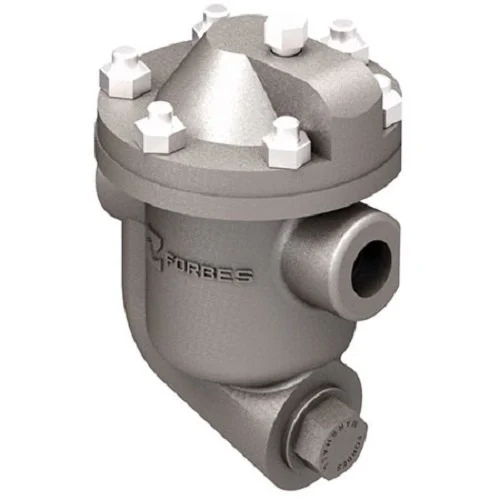
\includegraphics[width=0.8\textwidth,height=0.33\textheight,keepaspectratio]{figs/lastmin/bucket_trap.png}
    \caption{Bucket Trap}
    \label{fig:bucket_trap}
\end{figure}

\textbf{Features:}
\begin{enumerate}
    \item Resistance to water hammer.
    \item Suitable for high-pressure applications.
    \item Built-in strainer screen to prevent debris.
\end{enumerate}

\subsection{Types of Control Valves}

\subsubsection{Globe Valves}

\textbf{Description:} Globe valves are widely used for regulating flow in a pipeline. They offer good shutoff capability and are suitable for throttling services.

\textbf{Features:}
\begin{enumerate}
    \item Precise flow control.
    \item Low leakage rates.
    \item Suitable for high-pressure applications.
    \item Available in various sizes and materials.
\end{enumerate}
\subsubsection{Ball Valves}

\textbf{Description:} Ball valves are known for their durability and ability to provide tight shutoff. They are used in applications requiring quick on/off control.

\begin{figure}[h]
    \centering
    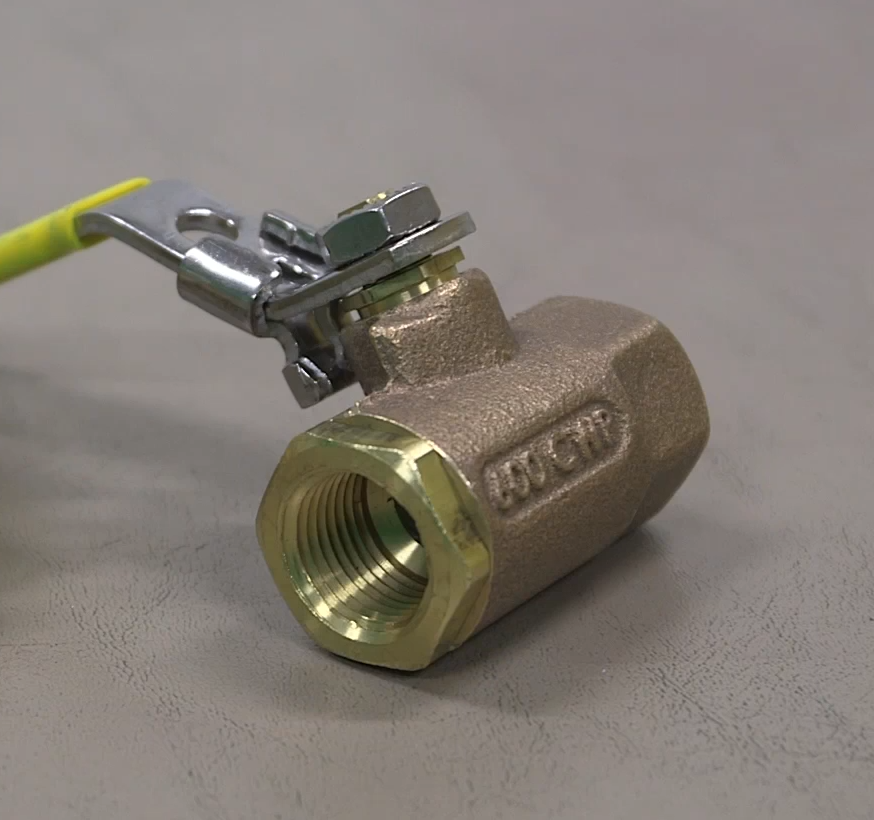
\includegraphics[width=0.8\textwidth,height=0.33\textheight,keepaspectratio]{figs/valves/ball.png}
    \caption{Ball Valve}
    \label{fig:ball_valve}
\end{figure}

\textbf{Features:}
\begin{enumerate}
    \item Quick operation with a quarter-turn movement.
    \item Minimal pressure drop when fully open.
    \item Suitable for high-temperature and high-pressure applications.
    \item Available in various configurations, such as two-way and three-way.
\end{enumerate}
\subsubsection{Butterfly Valves}

\textbf{Description:} Butterfly valves are used for regulating and isolating flow in pipelines. They are lightweight and offer a compact design.

\begin{figure}[h]
    \centering
    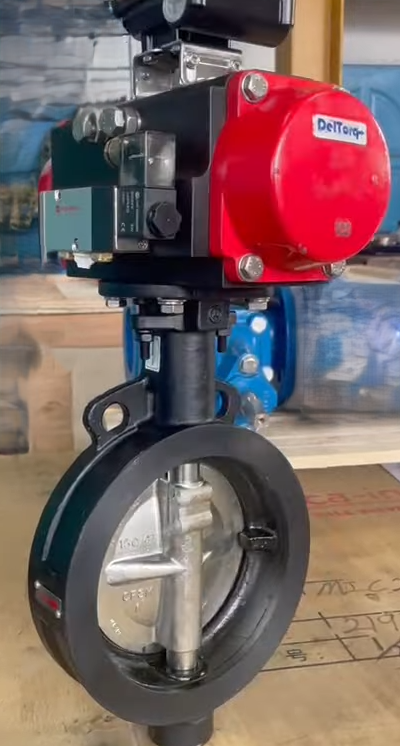
\includegraphics[width=0.8\textwidth,height=0.33\textheight,keepaspectratio]{figs/valves/butterfly.png}
    \caption{Butterfly Valve}
    \label{fig:butterfly_valve}
\end{figure}

\textbf{Features:}
\begin{enumerate}
    \item Quick operation with a quarter-turn movement.
    \item Low cost and maintenance.
    \item Suitable for large valve applications.
    \item Available in various materials to handle different types of fluids.
\end{enumerate}

\subsubsection{Diaphragm Valves}

\textbf{Description:} Diaphragm valves are used in applications requiring corrosion resistance and tight shutoff. They are ideal for handling slurries and viscous fluids.

\textbf{Features:}
\begin{enumerate}
    \item Leak-proof sealing.
    \item Suitable for abrasive and corrosive fluids.
    \item Easy to maintain and repair.
    \item Available in various materials, including rubber and plastic linings.
\end{enumerate}
\subsubsection{Check Valves}

\textbf{Description:} Check valves are designed to allow flow in one direction and prevent backflow. They are essential for protecting equipment and maintaining system integrity.

\textbf{Features:}
\begin{enumerate}
    \item Simple operation without the need for manual intervention.
    \item Low-pressure drop.
    \item Available in various types, such as swing check and lift check valves.
    \item Suitable for horizontal and vertical installations.
\end{enumerate}

\subsubsection{Control Valves}

\textbf{Description:} Control valves are used to regulate flow, pressure, temperature, and fluid level in industrial processes. They are critical for process automation.

\textbf{Features:}
\begin{enumerate}
    \item Precise control of process variables.
    \item Integration with control systems for automation.
    \item Available in various types, including linear and rotary motion control valves.
    \item Suitable for a wide range of applications and operating conditions.
\end{enumerate}